%%%%%%%%%%%%%%%%%%%%%%%%%%%%%%%%%%%%%%%%%
% Short Sectioned Assignment LaTeX Template Version 1.0 (5/5/12)
% This template has been downloaded from: http://www.LaTeXTemplates.com
% Original author:  Frits Wenneker (http://www.howtotex.com)
% License: CC BY-NC-SA 3.0 (http://creativecommons.org/licenses/by-nc-sa/3.0/)
%%%%%%%%%%%%%%%%%%%%%%%%%%%%%%%%%%%%%%%%%

%----------------------------------------------------------------------------------------
%	PACKAGES AND OTHER DOCUMENT CONFIGURATIONS
%----------------------------------------------------------------------------------------

\documentclass[paper=a4, fontsize=11pt]{scrartcl} % A4 paper and 11pt font size

% ---- Entrada y salida de texto -----

\usepackage[T1]{fontenc} % Use 8-bit encoding that has 256 glyphs
\usepackage[utf8]{inputenc}
%\usepackage{fourier} % Use the Adobe Utopia font for the document - comment this line to return to the LaTeX default

% ---- Idioma --------

\usepackage[spanish, es-tabla]{babel} % Selecciona el español para palabras introducidas automáticamente, p.ej. "septiembre" en la fecha y especifica que se use la palabra Tabla en vez de Cuadro

% ---- Otros paquetes ----

\usepackage{url} % ,href} %para incluir URLs e hipervínculos dentro del texto (aunque hay que instalar href)
\usepackage{amsmath,amsfonts,amsthm} % Math packages
%\usepackage{graphics,graphicx, floatrow} %para incluir imágenes y notas en las imágenes
\usepackage{graphics,graphicx, float} %para incluir imágenes y colocarlas
\usepackage{epstopdf}

% Para hacer tablas comlejas
%\usepackage{multirow}
%\usepackage{threeparttable}

%\usepackage{sectsty} % Allows customizing section commands
%\allsectionsfont{\centering \normalfont\scshape} % Make all sections centered, the default font and small caps

\usepackage{fancyhdr} % Custom headers and footers
\pagestyle{fancyplain} % Makes all pages in the document conform to the custom headers and footers
\fancyhead{} % No page header - if you want one, create it in the same way as the footers below
\fancyfoot[L]{} % Empty left footer
\fancyfoot[C]{} % Empty center footer
\fancyfoot[R]{\thepage} % Page numbering for right footer
\renewcommand{\headrulewidth}{0pt} % Remove header underlines
\renewcommand{\footrulewidth}{0pt} % Remove footer underlines
\setlength{\headheight}{13.6pt} % Customize the height of the header

\numberwithin{equation}{section} % Number equations within sections (i.e. 1.1, 1.2, 2.1, 2.2 instead of 1, 2, 3, 4)
\numberwithin{figure}{section} % Number figures within sections (i.e. 1.1, 1.2, 2.1, 2.2 instead of 1, 2, 3, 4)
\numberwithin{table}{section} % Number tables within sections (i.e. 1.1, 1.2, 2.1, 2.2 instead of 1, 2, 3, 4)

\setlength\parindent{0pt} % Removes all indentation from paragraphs - comment this line for an assignment with lots of text

\newcommand{\horrule}[1]{\rule{\linewidth}{#1}} % Create horizontal rule command with 1 argument of height


%----------------------------------------------------------------------------------------
%	TÍTULO Y DATOS DEL ALUMNO
%----------------------------------------------------------------------------------------

\title{	
\normalfont \normalsize 
\textsc{\textbf{Curso 2016-2017} \\ Grado en Ingeniería Informática \\ Universidad de Granada} \\ [25pt] % Your university, school and/or department name(s)
\horrule{0.5pt} \\[0.4cm] % Thin top horizontal rule
\huge Documentación práctica 1 TSI: \\Robot deambulador con ROS y Gazebo \\ % The assignment title
\horrule{2pt} \\[0.5cm] % Thick bottom horizontal rule
}

\author{Carlos Manuel Sequí Sánchez} % Nombre y apellidos

\date{\normalsize\today} % Incluye la fecha actual

%----------------------------------------------------------------------------------------
% DOCUMENTO
%----------------------------------------------------------------------------------------

\begin{document}

\maketitle % Muestra el Título

\begin{figure}[H] %con el [H] le obligamos a situar aquí la figura
	\centering
	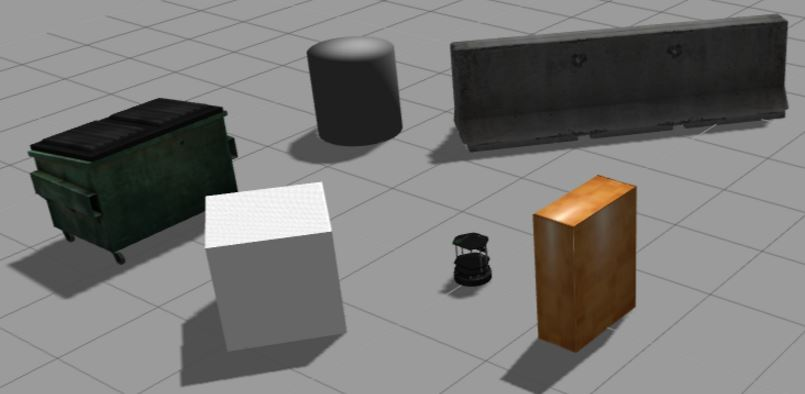
\includegraphics[scale=0.7]{1} 
\end{figure}

\newpage %inserta un salto de página

\tableofcontents % para generar el índice de contenidos

\newpage



\section{Primeros pasos}

Lo primero que hice de todo para la realización de la práctica fue crear un nuevo paquete ROS denominado random\_walk tal y como se indica en el guión. Tras haber solucionado un par de problemas que me surgieron con este tema, comencé analizando el código stopper.cpp y stopper.h, dado que basándonos en él prácticamente está montado el esqueleto del código a realizar.
\\ \\
Una vez analizado y comprendido el código proporcionado, la idea de resolución era sencilla: el robot anda hacia alante y, cuando encuentra un obstáculo (cosa que ya estaba implementada) simplemente calcula un número aleatorio analiza hacia donde hay una menor cantidad de obstáculos, gira hacia allí y reanuda la marcha (en caso de no haber más obstáculos). \\
\\
\section{Cambios realizados sobre el código stopper.cpp}

Lo primero que he modificado del código ha sido el método startMoving, el cual solo tenia en cuenta la acción de ir hacia alante con el booleano ''keepMoving''. Simplemente he añadido un condicional if-else para que, en caso de que no pueda avanzar, gire hacia algún lado.\\ \\
Tras ello me fuí al método scanCallBack y realicé los cambios para el mismo propósito, es decir, he incorporado un if-else para que una vez que (dentro de ese método) se ha comprobado que hay un obstáculo enfrente del turtlebot con el escaneo del laserscan, entonces llame a un método creado por mí el cual analiza cual de los dos lados es más conveniente para realizar el giro (método ChooseTurningSide). En caso de no hbaer obstáculo, evidentemente continua su marcha en linea recta.\\\\
Por último, como modificación también puede decirse que he añadido unos cuantos atributos de estado (booleanos) a la clase, por lo que los he inicializado en el constructor.

\newpage

\section{Métodos añadidos a la clase}

A continuación paso a explicar los únicos dos métodos que he visto conveniente agregar a la clase:
\\
\begin{itemize}
	\item \textbf{ChooseTurningSide(escaneo\_turtlebot, minIndex, maxIndex)}:
		\begin{itemize}
			\item Recibimos como parámetros el escáner del turtlebot y los índices mínimo y máximo del sensor de proximidad.
			\item En un solo bucle ''for'' condensamos dos análisis:
				\begin{itemize}
					\item Cantidad de obstáculos que hay a la derecha, utilizando el vector ''ranges'' el cual nos dice si hay objeto o no a la distancia asignada al sensor turtlebot. Para analizar la parte derecha recorremos el vector desde minIndex hasta maxIndex/2.
					\item Cantidad de obstáculos que hay a la izquierda, de la misma manera que para los de la derecha, pero esta vez recorriendo el vector desde maxIndex/2 hasta el final.
				\end{itemize}
			\item Una vez tenemos en 2 variables cuantos objetos hay a la izquierda y cuantos a la derecha, simplemente activamos una variable de estado ''leftTurning'' en caso de que haya más obstáculos a la derecha, o activamos ''rightTurning'' en el caso contrario.
		\end{itemize}
	

	\item \textbf{Turning()}
		\begin{itemize}
			\item Lo primero que hago es calcular un valor aleatorio entre 5 y 25, el cual hará que el robot gire durante una cantidad de tiempo aleatoria (''randTurningValue'').
			\item En función de la variable de estado activada en el método anterior, la velocidad angular será negativa (para un giro hacia la derecha) o positiva (para un giro hacia la izquierda).
			\item Como último, tras conocer hacia donde conviene girar, solo nos queda realizar el giro en sí, cosa de la que se encarga el publisher con el mensaje:\\ msg.angular.z = <<sentido\_giro>> * <<cantidad\_aleatoria>>
		\end{itemize}
\end{itemize}


Una vez realizado dicho giro hasta donde no se hayan obstáculos y, teniendo en cuenta todas las variables de estado pertinentes, el turtlebot continua su deambulación por el mapa.\\
Por último he añadido una línea al fichero launch con el fin de indicar desde ahí la distancia a la que turtlebot ha de detectar si hay o no obstáculos delante suya. Esta es la línea añadida: \\
<node name=''walker'' pkg=''random\_walk'' type=''walker'' args=''0.8'' output=''screen''/> \\
Con el parámetro ''args'' le indico que pasamos al programa como argumento el valor 0.8, para así recogerlo en el main con arg[1] y usarlo como distancia mínima de proximidad a un objeto.


\newpage
%------------------------------------------------

\bibliography{citas} %archivo citas.bib que contiene las entradas 
\bibliographystyle{plain} % hay varias formas de citar




\end{document}
